% !TeX program = lualatex
% !TeX encoding = utf8
% !TeX spellcheck = uk_UA

\documentclass[]{beamer}
\usetheme{PlasmaPhysics}
\usepackage{PlasmaPhysics}

\NewDocumentCommand{\E}{}{\vec{E}}
\NewDocumentCommand{\B}{}{\vec{B}}
\NewDocumentCommand{\J}{}{\vec{j}}
\NewDocumentCommand{\V}{}{\vec{v}}

\NewDocumentCommand{\divg}{m}{\vec{\nabla}\cdot{#1}}
\NewDocumentCommand{\rot}{m}{\vec{\nabla}\times{#1}}
\NewDocumentCommand{\grad}{m}{\vec{\nabla}#1}
\NewDocumentCommand{\vecdot}{mm}{\left[#1\times#2\right]}
\NewDocumentCommand{\dt}{m}{\frac{\partial #1}{\partial t}}

\usepackage{subcaption}
\usepackage{mathtools}
\setlength{\abovedisplayskip}{3pt}
\setlength{\belowdisplayskip}{3pt}
\usetikzlibrary{decorations.pathreplacing}
\newtcolorbox{mysidebyside}[1][]{
    notitle, sidebyside, blanker,
    sidebyside align=center seam,
    halign=center,
    lefthand width=.5\textwidth,
    #1
}



\graphicspath{{pictures/}}
\title[Лекції з фізики плазми]{\bfseries\huge Плазма як рідина}
\subtitle{\bfseries Лекції з фізики плазми}
\author{Пономаренко С. М.}
\date{}
% https://www.youtube.com/watch?v=zv9Y7YmHyBk
\def\stext#1{\text{
        \makebox[0pt]{
            \tikz[baseline] {\node[text width=50pt, align=center, execute at begin node=\setlength{\baselineskip}{-0.5ex}, blue] {#1};}
        }
}}


\begin{document}




%===============================================================================
\usebackgroundtemplate{
	\tikz\node[opacity=0.1]{\includegraphics[width=\paperwidth,height=\paperheight]{background}};%
}


\begin{frame}
	\thispagestyle{empty}
	\titlepage
\end{frame}


% ============================== Слайд ## ===================================
\begin{frame}{Гідродинаміка плазми}{}
	\begin{block}{}\justifying
        Під час руху $\vec{v}$ провідної рідини в магнітному полі $\B$:
        \begin{enumerate}
            \item в ній індукуються електричні поля $\E$ і виникають електричні струми $\J$;
            \item на струми в магнітному полі діє сила Ампера $\dfrac1c\vecdot{\V}{\B}$, яка істотно впливає на рух рідини $\vec{v}$;
            \item ці ж струми змінюють і саме магнітне поле $\B$.
        \end{enumerate}
        У результаті виникає складна картина взаємодії провідного середовища та електромагнітного поля. Для аналізу поведінки плазми необхідно розв'язувати самоузгоджену задачу.
	\end{block}
%	\begin{center}
%		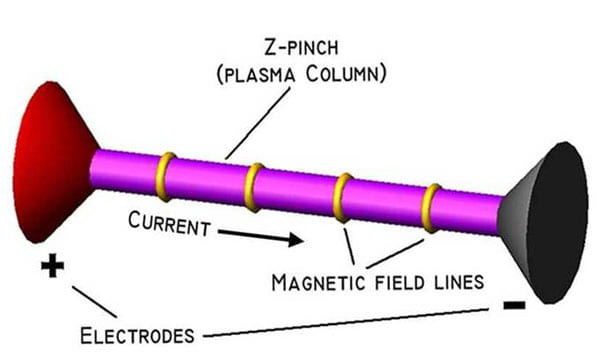
\includegraphics[width=0.5\linewidth]{zpinch}
%	\end{center}
\end{frame}
% ===========================================================================

% ============================== Слайд ## ===================================
\begin{frame}{Модель двох рідин}{}
	\begin{onlyenv}<1>
		\begin{block}{}\justifying
			Гідродинамічний опис в найпростішому випадку --- представлення плазми у вигляді суміші двох рідин --- електронної та іонної. Ці рідини взаємодіють між собою через \alert{зіткнення} та \alert{спільне електричне поле}. Такий опис називається дворідинною гідродинамікою.

			\bigskip

			Рівняння руху електронів та йонів:
			\begin{align*}
				Mn_i\left(\dt{\V_i} + (\V_i\cdot\nabla)\V_i \right) = Zen_i \left(\E + \frac1c \vecdot{\V_i}{\B} \right) - \grad{p_i} - \dot{\vec{P}}_{ie}, \\
				mn_e\left(\frac{\partial\vec{v}_e}{\partial t} + (\vec{v}_e\cdot\nabla)\vec{v}_e \right) = -en_e \left(\E + \frac1c \vecdot{\V_e}{\B}\right) -\grad{p_e} - \dot{\vec{P}}_{ei},
			\end{align*}де $\dot{\vec{P}}_{ie} = - \dot{\vec{P}}_{ei} = - \frac{mn}{\tau}(\vec{v}_i - \vec{v_e})$ --- зміни імпульсів через зіткнення іонів з електронами іонної та електронної рідин, відповідно (сила Брагінського).
		\end{block}
	\end{onlyenv}
	\begin{onlyenv}<2>
		\begin{block}{}\justifying
			Для отримання повної системи рівнянь дворідинної гідродинаміки слід доповнити:
			\begin{enumerate}
				\item рівняннями неперервності (збереження маси):
				      \begin{equation*}
					      \dt{n_i} + \divg{(n_{i}\V_i)} = 0, \quad
					      \dt{n_e} + \divg{(n_{e}\V_e)} = 0.
				      \end{equation*}
				\item рівняннями Максвелла:
				      \begin{alignat*}{2}
					      \divg{\B} & = 0, \quad                  &  & \rot{\E} = -\frac1c \dt{\B},                                         \\
					      \divg{\E} & = 4\pi e(Zn_i - n_e), \quad &  & \rot{\B} = \frac{4\pi e}{c}(Zn_i\vec{v}_i - n_e\V_e) + \frac1c \dt{\E}.
				      \end{alignat*}
			\end{enumerate}
		\end{block}
	\end{onlyenv}
\end{frame}

% ============================== Слайд ## ===================================
\begin{frame}{Однорідинна гідродинаміка}{}
	\begin{block}{}\justifying
		Найпростіший опис динаміки плазми дають рівняння однорідинної гідродинаміки. Наближення однорідинної гідродинаміки справедливе для опису \alert{повільних} (у масштабі періоду плазмових коливань) \alert{великомасштабних} (у масштабі дебаївського радіусу) рухів плазми, \alert{коли порушеннями електронейтральності можна знехтувати}.
		\begin{enumerate}
			\item $Zn_i \approx n_e$.
			\item $T = T_i = T_e$.
			\item $p = p_i + p_e = 2 n T$, $n$ --- концентрація іонів.
			\item $M \gg m$. Інерційністю електронів нехтуємо $m \approx 0$.
			\item Швидкість плазми як цілого ототожнюється з швидкістю іонів $\vec{v} \approx \vec{v}_i$.
		\end{enumerate}
	\end{block}
	\begin{equation*}
		\tcbhighmath{
			Mn\left(\dt{\V} + (\vec{v}\cdot\nabla)\vec{v} \right) = - \grad{p} + \frac1c\vecdot{\J}{\B}.
		}
	\end{equation*}
\end{frame}
% ===========================================================================


% ============================== Слайд ## ===================================
\begin{frame}{Узагальнений закон Ома}{}
	\begin{block}{}
		Виключаючи з розгляду електронну компоненту. ми вводимо в теорію окрему незалежну змінну --- густину струму $\J$.
		\begin{equation*}
			\frac12\nabla p = -en\E - \frac{en}c\vecdot{\V}{\B} + \frac1c \vecdot{\J}{\B} + \frac{en}{\sigma}\J,
		\end{equation*}
		де $\sigma = \frac{e^2n\tau}{m}$.
		\begin{equation*}
			\tcbhighmath{
				\J + \frac\sigma{nec} \vecdot{\J}{\B} -  \frac{\sigma}{nec}\nabla p_e = \sigma \E^*,
			}
		\end{equation*}
		де $\E^* = \E + \frac1c\vecdot{\V}{\B}$ --- електричне поле в супутній системі відліку (в системі, що рухається разом з плазмою).

		Доданок пропорційний $\vecdot{\J}{\B}$ відповідає струму Холла (див. \href{https://en.wikipedia.org/wiki/Hall_effect}{еффект Холла}).

	\end{block}

	\begin{block}{}
		При $\B = 0$ та $p = \const$ випливає, що
		\begin{equation*}
			\J = \sigma\E.
		\end{equation*}
	\end{block}
\end{frame}
% ===========================================================================


% ============================== Слайд ## ===================================
\begin{frame}{Провідність плазми}{}
	\begin{block}{}\justifying
		Обчислення провідності з кінетичних уявлень, було вперше виконано \href{https://en.wikipedia.org/wiki/Spitzer_resistivity}{Спітцером}, тому величину $\sigma$ називають провідністю Спітцера (Spitzer conductivity):
		\begin{equation*}
			\frac1{\sigma_{\parallel}}\left[\text{Ом}\cdot\text{м}\right] = 5.2\cdot10^{-5}Z\ln\Lambda \cdot T^{3/2}, \quad \sigma_{\parallel} \approx 1.96\sigma_{\perp}.
		\end{equation*}
		де $Z$ --- заряд іонів, $\ln\Lambda$ --- кулонівський логарифм.

		\begin{center}
			\begin{tblr}{
					colspec={cc},
					vlines,
					hlines,
				}                        & $T$, еВ & $n$, см\textsuperscript{-3} & $\ln\Lambda$ \\
				Лабораторна плазма       & $0.2$   & $10^{11}$                   & $10.2$       \\
				Плазмовий тор            & $100$   & $10^{13}$                   & $13.7$       \\
				Термоядерний реактор     & $10^4$  & $10^{18}$                   & $16.0$       \\
				Плазма лазерного синтезу & $10^3$  & $10^{24}$                   & $6.8$
			\end{tblr}
		\end{center}
	\end{block}
\end{frame}
% ===========================================================================

% ============================== Слайд ## ===================================
\begin{frame}{Система рівнянь однорідинної гідродинаміки}{}
	\begin{align*}
		\rho\left(\dt{\V} + (\V\cdot\nabla)\V \right) = - \grad{p} + \frac1c \vecdot\J\B, \\
		\J + \frac\sigma{nec}\vecdot\J\B -  \frac{\sigma}{nec}\grad{p_e} = \sigma \E^*,  \\
		\dt{n} + \divg{(n\V)} = 0.
	\end{align*}

	І рівняння Максвела (струмом зміщення порівняно з провідністю знехтуємо):
	\begin{alignat*}{2}
		\divg\B & = 0, \quad &  & \rot\E = -\frac1c \dt{B}, \\
		\divg\E & =0, \quad  &  & \rot\B = \frac{4\pi}{c}\J.
	\end{alignat*}
\end{frame}
% ===========================================================================

%\begin{frame}{Основне рівняння магнітної гідродинаміки плазми}
%\begin{columns}
%	\begin{column}{0.5\linewidth}
%         \begin{figure}\centering
%            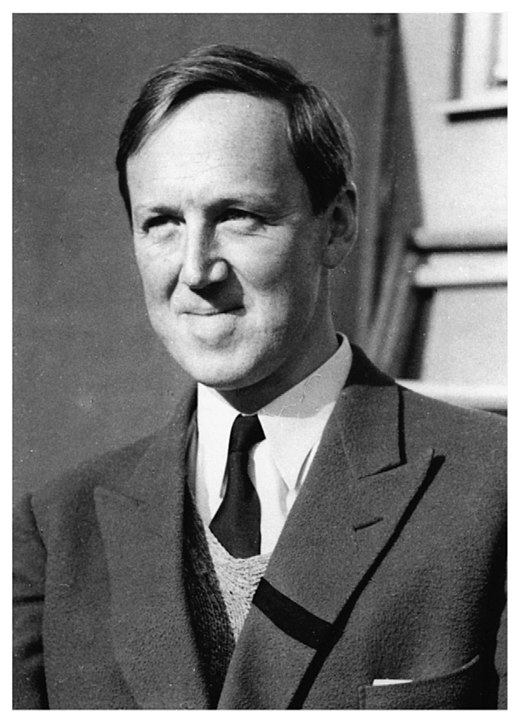
\includegraphics[width=0.5\linewidth]{pictures/YoungAlfven.jpg}
%
%            \caption*{\scriptsize Шведський фізик та астроном, лауреат Нобелівської премії з фізики 1970 року за внесок у розвиток магнітогідродинаміки. Фахівець у галузі космічних променів, прискорювачів електронів та електродинаміки. Розвинув теорії утворення полярного сяйва, геомагнітних бур, утворення Сонячної системи.}
%         \end{figure}
%	\end{column}
%	\begin{column}{0.5\linewidth}
%         \begin{block}{}\justifying
%        При розв'язанні системи диференціальних рівнянь її, як правило, намагаються звести до одного рівняння. Відповідно до цього поведінку плазми можна описувати, наприклад, полями концентрації або швидкості або полем густини струму.
%
%        \medskip
%
%        В багатьох випадках плазма знаходиться в магнітному полі, яке істотно впливає на рух частинок у напрямках, перпендикулярних до цього поля.
%
%        \medskip
%
%        Ідея Альвена тому, щоб описувати динаміку плазми в наближенні однорідинної гідродинаміки через магнітні поля.
%        \end{block}
%	\end{column}
%\end{columns}
%
%\end{frame}

% ============================== Слайд ## ===================================
\begin{frame}{Магнітний тиск}{}
	\begin{block}{}\justifying
		Рівняння руху плазми
		\begin{equation*}
			\frac{d\vec{v}}{d t}  = - \frac1\rho\nabla p + \frac1{4\pi\rho}
        \vecdot{\left[\rot\B\right]}{\B}.
		\end{equation*}
		Формула векторного аналізу: \(
		\vecdot{\left[\rot\B\right]}{\B} = (\B\cdot\nabla)\B - \nabla\dfrac{B^2}2
		\).
		\begin{equation*}
			\frac{d\vec{v}}{d t}  = - \frac1\rho\nabla\left( p + \frac{B^2}{8\pi}\right) +  \frac1{4\pi\rho}(\B\cdot\nabla)\B
		\end{equation*}
		Розділимо рівняння на перпендикулярну і поперечну (по відношенню до магнітного поля) компоненти:
		\begin{equation*}
			\frac{d\vec{v}_{\perp}}{d t}      = - \frac1\rho\nabla\left( p + \frac{B^2}{8\pi}\right), \quad 	\frac{d\vec{v}_{\parallel}}{d t}  = \frac1{4\pi\rho}(\B\cdot\nabla)\B .
		\end{equation*}

		На плазму може впливати сила магнітного тиску $ \frac{B^2}{8\pi} $. Тобто, плазму можна утримувати магнітною стінкою, штовхати магнітним поршнем; плазмові згустки можна вистрілювати з магнітної гармати.
	\end{block}
\end{frame}
% ===========================================================================

%% ============================== Слайд ## ===================================
\begin{frame}{Ідеальна провідність плазми}{}
	\begin{block}{}\justifying
		Плазма характеризується високою провідністю.
		Використаємо наближення $\sigma \to \infty$. В цьому випадку як завгодно мале електричне поле викликало б
		нескінченний струм, що вимагало б нескінченно великої витрати енергії і тому неможливе. Отже, в  наближенні ідеальної провідності електричне поле $\E^* = 0$, звідки:
		\begin{equation*}
			\E = -\frac1c \vecdot{\V_{\perp}}{\B}.
		\end{equation*}
	\end{block}
\end{frame}
%% ===========================================================================


% ============================== Слайд ## ===================================
\begin{frame}{Вмороженість магнітного поля}{}
	%\begin{block}{}
	%   Ефект полягає в тому, що магнітні силові лінії переміщуються разом із плазмою.
	%\end{block}
	\begin{onlyenv}<1>
		\begin{block}{}
			Використаємо рівняння:
			\begin{align*}
				\E                          & = -\frac1c \vecdot{\V_{\perp}}{\B}, \\
				\rot\E          & = -\frac1c \dt{\B},       \\
				\frac{\partial \rho}{\partial t} & = - \vec\nabla\cdot(\rho\vec{v}).
			\end{align*}
			І формулу векторного аналізу \(\rot{\vecdot{\vec{A}}{\B}} = \left( \B\cdot\vec{\nabla}\right)\vec{A} - \left( \vec{A}\cdot\vec{\nabla}\right)\B + 	\vec{A}\  \divg\B - \B\ \divg{\vec{A}} \)
		\end{block}
	\end{onlyenv}

	\begin{onlyenv}<1->
		\begin{block}{}
			%Отримаємо:
			\begin{equation*}
				\tcbhighmath{
					\frac{d}{dt}\left(\frac{\B}{\rho}\right) = \left(\frac{\B}{\rho}\vec{\nabla}\right)\vec{v}.
				}
			\end{equation*}
		\end{block}
	\end{onlyenv}

	\begin{onlyenv}<2>
		\begin{block}{}
			Коли швидкість змінюється тільки \alert{в напрямку, перпендикулярному
				до магнітного поля:}
			\begin{equation*}
				\frac{\B}{\rho} = \const.
			\end{equation*}
			\begin{enumerate}\scriptsize
				\item Густина силових ліній, тобто індукція магнітного поля, змінюється пропорційно до  густини речовини.
				\item Під час руху плазми лінії магнітного поля не можуть розриватисяся або перез'єднуватися. Іншими словами, в рамках ідеальної магнітної гідродинаміки зміна топології магнітного поля неможлива.
				\item Зміна магнітного поля в нерухомій плазмі стає неможливою: така зміна породжує сильні струми, що компенсують початкову зміну магнітного поля. В результаті магнітне поле в плазмі може змінюватися тільки в процесі руху самої плазми.
				\item Ефективний показник адіабати для магнітного тиску $\gamma_{\perp} = 2$, тобто під час плоского стиснення поперек поля магнітний тиск зростає швидше, ніж тиск ідеального газу.
			\end{enumerate}
		\end{block}
	\end{onlyenv}

	\begin{onlyenv}<3>
		\begin{block}{}\scriptsize
			\alert{При плоскому стисненні вздовж магнітного поля} рівняння дає:
			\begin{equation*}
				\B = \const.
			\end{equation*}
			При плоскому стисненні плазми вздовж магнітного поля індукція та магнітний тиск
			залишаються постійними: $\gamma_{\parallel} = 0$. Так і має бути згідно з уявленням про вморожене поле: при плоскому стисненні уздовж поля силові лінії тільки скорочуються в довжину, але не згущуються.
		\end{block}
	\end{onlyenv}

	\begin{onlyenv}<3>
		\begin{block}{}\scriptsize
			\alert{При ізотропному стисненні речовини} рівняння дає:
			\begin{equation*}
				B \propto \rho^{2/3}.
			\end{equation*}
			Ефективний показник адіабати для магнітного тиску при ізотропному стисненні: $\gamma= \frac43$. Як відомо, таке саме значення показника адіабати і для тиску електромагнітного випромінювання.
			%
			%			\bigskip
			%
			%			Закон наростання магнітного поля при ізотропному стисненні має велике значення в астрофізиці, зокрема в теорії утворення зірок за допомогою гравітаційної конденсації космічної плазми. При цьому напруженість вморожених у плазму полів зростає пропорційно до густини в степені $2/3$, і доводиться вводити спеціальні механізми витіснення поля, щоб пояснити, чому зірки, що утворюються, не володіють колосальними магнітними полями.
		\end{block}
	\end{onlyenv}
\end{frame}
% ===========================================================================

% ============================== Слайд ## ===================================
\begin{frame}{Дифузія магнітного поля}{}
	\begin{onlyenv}<1>
		\begin{block}{}
			Якщо врахувати скінченну провідність, то у системі координат, пов'язаній із плазмою, діятимуть електричні поля, що викликають електричні струми:
			\begin{equation*}
				\J = \sigma\left(\E  + \frac1c \vecdot{\V_{\perp}}{\B}\right).
			\end{equation*}
			Підставимо вираз в рівняння Максвелла \(\J = \frac{c}{4\pi}\, \rot\B\):
			\begin{equation*}
				\E  + \frac1c\vecdot{\V_{\perp}}{\B} = \frac{c}{4\pi\sigma}\, \rot\B.
			\end{equation*}
			Виконаємо операцію  взяття ротора з обох частин цього рівняння і використаємо рівняння \( \rot\E = - \frac1c\dt{\B}\):
			\begin{equation*}
				\dt{\B} = \rot{\vecdot{\V}{\B}} + \frac{c}{4\pi\sigma}\nabla^2\B.
			\end{equation*}
			Це рівняння відрізняється від рівняння вмороженого поля доданком з~$\nabla^2\B$.
		\end{block}
	\end{onlyenv}
	\begin{onlyenv}<2>
		\begin{block}{}\justifying\scriptsize
			Розглянемо випадок, коли рух речовини відсутній $\vec{v} = 0$:
			\begin{equation*}
				\frac{\partial \B}{\partial t} = \frac{c}{4\pi\sigma}\nabla^2\B.
			\end{equation*}
			Це рівняння тотожне за виглядом із рівнянням дифузії. Роль коефіцієнта дифузії відіграє величина:
			\begin{equation*}
				D = \frac{c}{4\pi\sigma}.
			\end{equation*}
			Можна сказати, що через кінцеву провідність магнітне поле ніби просочується крізь плазму за дифузійним
			законом із коефіцієнтом дифузії~$D$.

			Глибина просочування:
			\begin{equation*}
				\delta = \sqrt{Dt}.
			\end{equation*}
			Для періодичного процесу час $t$ порядку зворотної  частоти $1/\omega$. Величину називають товщиною \alert{скін-шару}:
			\begin{equation*}
				\delta = \frac{c}{4\pi\sigma\omega}
			\end{equation*}
			Магнітне поле, а разом з ним і змінний струм проникає в плазму тільки в результаті дифузії. Але струм тече лише в тонкому поверхневому шарі провідника, який називають \alert{скін-шаром}.
		\end{block}
	\end{onlyenv}
\end{frame}
% ===========================================================================

\end{document}

